\documentclass[a4paper,10pt]{article}
\usepackage[utf8]{inputenc}
\usepackage{graphicx}
\usepackage{amsmath}
\usepackage{amssymb}
\usepackage{amsthm}
\usepackage{booktabs}
\usepackage{caption}
\usepackage{geometry}
%\usepackage{hyperref}
\usepackage{makeidx}
\usepackage{microtype}
\usepackage{subfig}
\usepackage{tabularx}
\usepackage{url}
\usepackage{varioref}
\usepackage{xcolor}
\usepackage{multicol}
\usepackage[italian]{babel}
\usepackage{mathtools}
\usepackage{booktabs}
\usepackage{multirow}
\usepackage{verbatim}
\usepackage{float}


\addto\captionsenglish{
  \renewcommand{\contentsname}%
    {Indice}%
}



\title{Laboratorio I: Misura di $g$ con una molla \\ Analisi della dipendenza del periodo e l'allungamento dalla massa\\
\begin{large}
Dipartimento di Fisica E.Fermi - Università di Pisa
\end{large}}

\author{Di Ubaldo Gabriele}
\date{}

\begin{document}

\maketitle

\section{Introduzione}
\subsection{Teoria}
\textbf{Obiettivo:} Misura dell’accelerazione di gravità $g$  a Pisa praticamente al livello del suolo a partire dagli allungamenti di una molla.\\
La legge di Hooke dice che:
\begin{equation}\label{hooke}
F_h=k(x-x_0)
\end{equation}
che in equilibrio diventa:
\begin{equation}\label{ho}
g(m_p+m_i+m_m/3)=k(l_i-l_0)
\end{equation}

Dove $m_p$ è la massa del piattello; $m_i$ è la massa posta sul piattello;$m_m $ è la massa della molla; $l_i$ la lunghezza della molla sotto carico; $l_0$ la lunghezza della molla a riposo.

Il periodo di oscillazione della molla è invece dato da:
\begin{equation}\label{periodo}
T_i^2=\frac{4\pi^2}{k}(m_i+m_p+m_m/3)
\end{equation}


\subsection{Apparato sperimentale}
\begin{itemize}
\item{Molla $m_m=7.944g $e piattello $m_p=7.771g$}
\item{Cronometro di risoluzione $0.01s$}
\item{Bilancia di precisione di risoluzione $0.001g$}
\item{Metro a nastro di risoluzione $1mm$}
\item{Pesetti di masse $5g;10g;20g;50g$}
\end{itemize}



\section{Esperimento}
\subsection{Acquisizione misure}
Abbiamo controllato che il valore dichiarato dei pesetti fosse corretto con la bilancia di precisione, osservando che il disaccordo con il valore nominale poteva essere trascuraato rispetto all'incertezza maggiore sulle lunghezze. Per semplicità abbiamo utillizzato il valore nominale dei pesi.
La lunghezza a riposo della molla è $l_0=12.4\pm0.1cm$.
Abbiamo attaccato il piattelo, posto le diverse masse su di esso e per ognuna di queste è stata misurata la lunghezza complessiva.
Per ciascuna massa sono state effettuate 5 misure di 10 oscillazioni ognuna. $\tau=10T$ si riferisce a 10 oscillazioni\\

I risultati ottenuti sono descritti dalle seguenti tabelle:
\begin{table}[H]
\centering
\caption{Allungamenti acquisiti}
\label{my-label}
\begin{tabular}{c|c|c}
$m(g)$ & \multicolumn{1}{l|}{$l(cm)$} & $l-l_0(cm)$ \\ \hline
5    & 17.6                          & 5.2        \\
10   & 19.7                          & 7.3        \\
15   & 21.5                          & 9.1        \\
20   & 23.6                         & 11.2       \\
25   & 25.6                         & 13.2       \\
30   & 27.6                         & 15.2       \\
35   & 29.5                         & 17.1       \\
40   & 31.5                         & 19.1       \\
45   & 33.6                         & 21.2       \\
50   & 35.5                         & 23.1      
\end{tabular}
\end{table}

\begin{table}[!htb]
\centering
\caption{Periodi acquisiti}
\label{my-label}
\begin{tabular}{c|ccccc}
$m(g)$ & \multicolumn{5}{c|}{$\tau_i(s)$}  \\ \hline
5    & 5.13 & 4.89  & 4.96 & 4.87 & 4.89 \\
10   & 5.75 & 5.67  & 5.74 & 5.83 & 5.73 \\
15   & 6.41 & 6.43  & 6.31 & 6.35 & 6.37 \\
20   & 6.97 & 6.91  & 7.01 & 6.99 & 7.04 \\
25   & 7.65 & 7.49  & 7.50 & 7.47 & 7.61 \\
30   & 8.00 & 8.02  & 8.07 & 7.96 & 8.03 \\
35   & 8.52 & 8.54  & 8.50 & 8.40 & 8.59 \\
40   & 8.95 & 8.92  & 9.02 & 8.97 & 8.91 \\
45   & 9.24 & 9.35  & 9.34 & 9.22 & 9.47 \\
50   & 9.80 &10.01  & 9.82 & 9.92 & 9.85
\end{tabular}
\end{table}


\subsection{Analisi dei dati}
Intuitivamente vediamo che per un aumento di $5g$ vi è circa un aumento di $2cm$ il che conferma in prima analisi la legge di Hooke.
Partendo dai risultati delle misurazioni è stata calcolata la media $m_{\tau}$ del periodo di 10 oscillazioni.
Dopodichè è stata ricavata la misura di $k$. 

\begin{table}[!htb]
\centering
\caption{Analisi dei periodi}
\label{my-label}
\begin{tabular}{llll}
$m(g)$ & $\tau_i(s)$ & $T_i(s)$      & $T_i^2(s)$    \\
5      & 4.95 $\pm$ 0.05 & 0.495$\pm$ 0.005 & 0.245 $\pm$ 0.005 \\
10     & 5.74 $\pm$ 0.02 & 0.574$\pm$ 0.002 & 0.329 $\pm$ 0.003 \\
15     & 6.37 $\pm$ 0.02 & 0.637$\pm$ 0.002 & 0.406 $\pm$ 0.003 \\
20     & 6.98 $\pm$ 0.05 & 0.698$\pm$ 0.005 & 0.487 $\pm$ 0.003 \\
25     & 7.55 $\pm$ 0.03 & 0.755$\pm$ 0.003 & 0.570 $\pm$ 0.005 \\
30     & 8.02 $\pm$ 0.04 & 0.802$\pm$ 0.004 & 0.643 $\pm$ 0.003 \\
35     & 8.49 $\pm$ 0.02 & 0.849$\pm$ 0.002 & 0.721 $\pm$ 0.003 \\
40     & 8.95 $\pm$ 0.02 & 0.895$\pm$ 0.002 & 0.801 $\pm$ 0.004 \\
45     & 9.32 $\pm$ 0.05 & 0.932$\pm$ 0.005 & 0.869 $\pm$ 0.009 \\
50     & 9.88 $\pm$ 0.04 & 0.988$\pm$ 0.004 & 0.976 $\pm$ 0.008
\end{tabular}
\end{table}
\pagebreak
Per l'errore su $T_i^2$ abbiamo usato l'espansione in serie di Taylor per più variabili.

\subsubsection{Stima di $k$}
Il seguente grafico descrive la proporzionalita tra la massa e il periodo quadro:

\begin{figure}[!htb]
\begin{center}
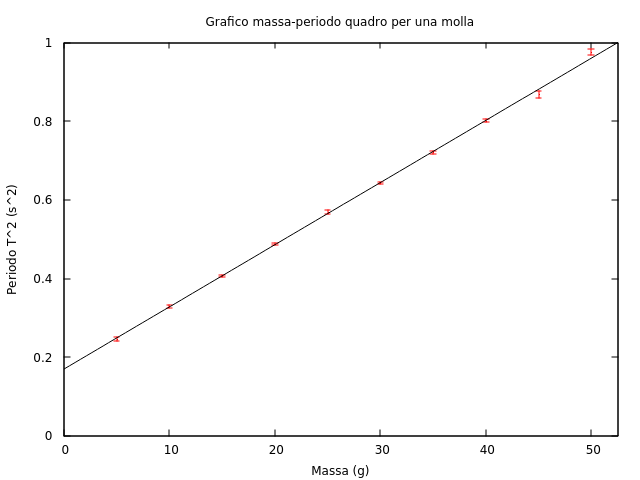
\includegraphics[width=10cm]{/home/zerch/Documents/UNIPI/LAB1/2Molla/Grafici/graf-m-T2.png}
\end{center}
\end{figure}
Abbiamo fatto un fit lineare attraverso gnuplot (il proramma usa l'algoritmo di Marquardt-Levenberg) e calcolato il $\chi^2$
L'intercetta del fit $f(x)=ax+b$ è $-b/a\approx -10.5g$ che è compatibile con $(m_p+m_m/3)$.
Per determinare la costante della molla usiamo $a=4\pi^2/k$ e otteniamo: 
\begin{equation}
k=2.46\pm0.02 N/m
\end{equation}
I risultati del fit sono:
\begin{equation}
 \chi^2=8.32  \quad \chi^2_r=1.04 \quad  a=0.0158\pm0.66\%	\quad  b=0.169\pm 1.62
\end{equation}



\subsubsection{Stima di $g$}
Il seguente grafico mostra la dipendenza tra la massa e l'allungamento.
\begin{figure}[!htb]
\begin{center}
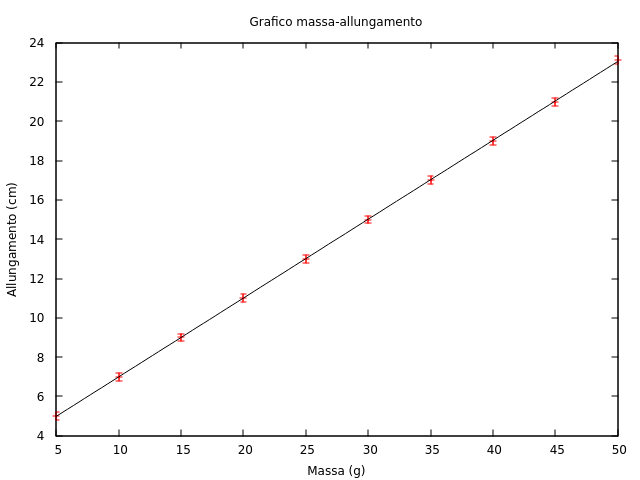
\includegraphics[width=10cm]{/home/zerch/Documents/UNIPI/LAB1/2Molla/Grafici/graf-m-l.png}
\end{center}
\end{figure}
La retta di fit interseca l'asse delle ascisse in $-b/a\approx7.45$ che è compatibile con la massa del piattello non considerata nel grafico.
I risultati del fit sono:
\begin{equation}
\chi^2=0.16 \quad \chi^2_r=0.02 \quad a=0.4\pm0.16\% \quad b=0.02\pm0.66\%
\end{equation}
Il coefficiente angolare della retta è $g/k$
Quindi 
\begin{equation}
g=9.84\pm 0.09 m/s2
\end{equation}


\section{Conclusione}
 Il valore del $\chi^2$ per le due rette di fit conferma  la validità del modello fisico utilizzato per il comportamento della molla. La stima di $g$ è in ottimo accordo con il valore dichiarato per Pisa di $g=9.807$ che rientra nell'errore della nostra misura. Il fatto che il $\chi^2$ sia così basso nel secondo fit può voler dire che abbiamo sovrastimato l'errore e in realtà i nostri strumenti hanno una precisione maggiore di quella attribuita.
\end{document}






